
\section{Detachment on MAST}
detachment, power balance, radiation front location, XPR literature on MASTU



\section{IRVB concept}
The IRVB is the diagnostic that was developed as part of the PhD project and will be used to gain scientific understanding.
The currently more established method to measure the energy radiated from the plasma is through resistive bolometers. A thin layer of absorbent material is exposed to the radiation and its temperature increase. This is measured via the change in resistivity of a resistor attached on the back of the foil. Each detector can measure the radiation for only one line of sight (LOS), so usually an array of detectors is present to measure the radiation across one plane. Tomographic reconstruction is then used to get the radiation profile from the line integrated values. This method is reliable and mature, but every LOS requires its own measuring apparatus and the resolution is limited by the number of sensors installed and how narrow the LOS is. A more recent approach expected to provide better resolution is the infra red video bolometer (IRVB). 

A thin foil is exposed to the plasma radiation through a pinhole so that each point of the foil corresponds to a different LOS. The foil heats up according to the radiation it receives and the change in temperature is measured via an infra red camera. The advantage relies in the very large number of LOS accessible with a single device and the capability to image very large or small portions of the plasma based on foil and pinhole relative position. The downside is the physics of thermal diffusion needs to be considered and it introduces a limit in the time resolution of the diagnostic. A sketch of the IRVB in MASTU is in \autoref{fig:IRVB_sketch}.

\begin{figure}
	\centering
	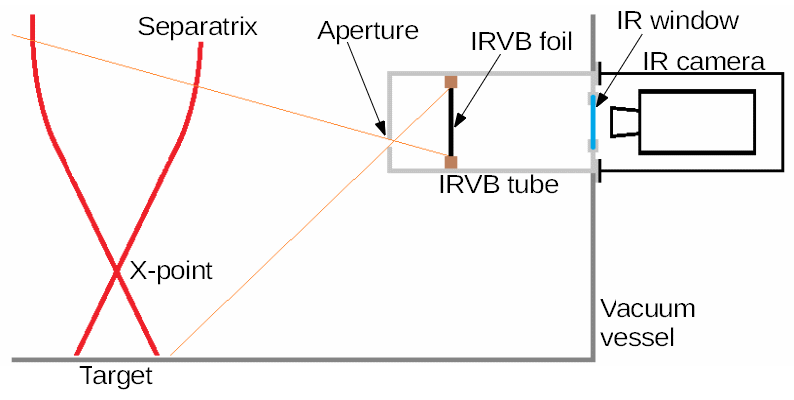
\includegraphics[width=\linewidth]{Chapters/chapter2/figs/IRVB cartoon.png}
	\caption{Schematic representation of the main components of a IRVB diagnostic}
	\label{fig:IRVB_sketch}
\end{figure}

There are various elements to consider in the design of the diagnostic.
The small thickness of the foil allows to treat the heat diffusion as a 2D problem and lower the thermal inertia, allowing for a higher temperature rise for given input power. The thickness must be anyway large enough for the vast majority of the radiation to be absorbed. The foil must also (if a significant amount of neutrons are produced) be made of a material weakly subject to neutron induced transmutation and vacuum compatible.\cite{Mukai2021}
It is important that the foil is blackened to reduce reflection of lower wavelengths, but this introduces the an interface between materials that might impede thermal transfer. The coating could, depending on the technique, be deposited non uniformly on the foil, adding to the non uniformity already present on the foil. The coating too must be stable and vacuum compatible. \cite{Mukai2016}
The infra red camera must be positioned as close as possible to the foil in order to increase the resolution and signal. If the neutron flux is significant or there are mechanical constraints mirrors or periscopes must be used. All apparatus must be suitable for infra red radiation and properly coated.
It has great importance in the design the positioning and size of the pinhole with respect of the foil. The distance and position will impact the field of view of the diagnostic, its spatial resolution and the radiation intensity. The size of the pinhole will impact the intensity and the resolution.\\
\hl{Previous implementations}


\section{MASTU implementation}

The IRVB system developed with this PhD project is a prototype designed with the aim to prove this technology in spherical tokamaks, first time this is done, measuring the radiation profile around the x-point. The design, shown in \autoref{fig:IRVB_components} is based on work previously done by M. L. Reinke for an IRVB system for NSTX-U.\cite{VanEden2016} The pinhole is located left and below the projection of the centre of the foil toward the center column, to aim the field of view at the lower x-point. The positioning of the IRVB tube can be seen in \autoref{fig:IRVB_location}. An approximate view inside MASTU as if the IRVB operates as a camera, to show the features and obstructions, is shown in \autoref{fig:calcam}.

\begin{figure}
	\centering
	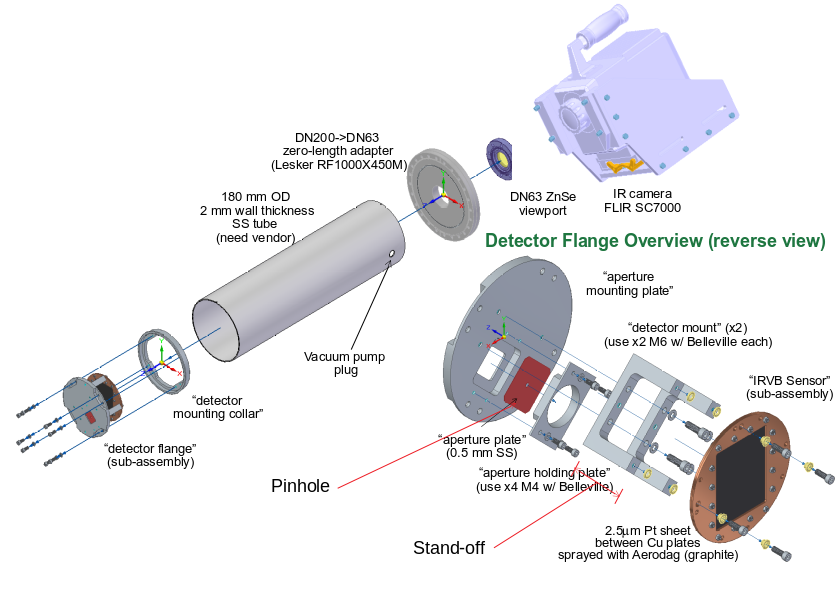
\includegraphics[width=\linewidth]{Chapters/chapter2/figs/IRVB2.png}
	\caption{IRVB components overview. To change pinhole size and foil pinhole distance the tube must be removed while the camera is always accessible. Adapted from \cite{Reinke2017a}}
	\label{fig:IRVB_components}
\end{figure}

\begin{figure}
	\centering
	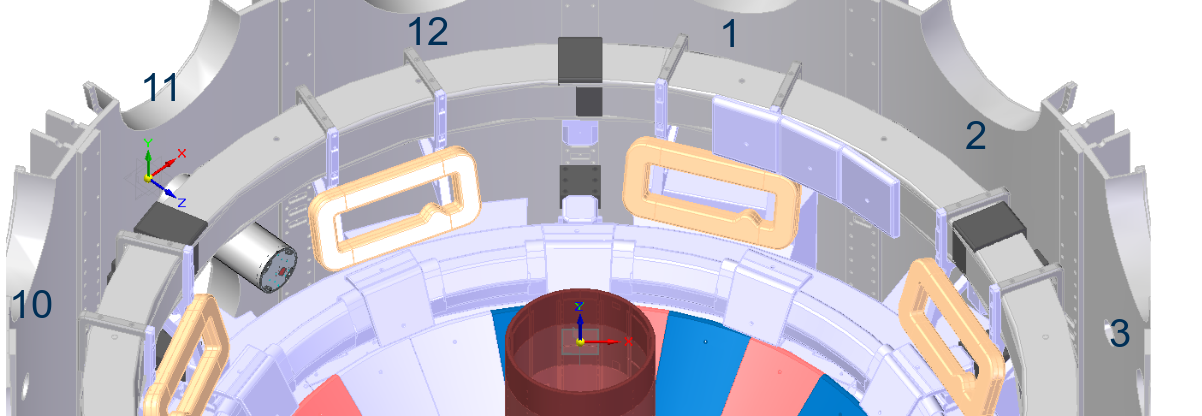
\includegraphics[width=\linewidth]{Chapters/chapter2/figs/where_irvb.png}
	\caption{Positioning of the IRVB inside the vacuum vessel of MASTU. Adapted from \cite{Reinke2017a}}
	\label{fig:IRVB_location}
\end{figure}

\begin{figure}
	\centering
	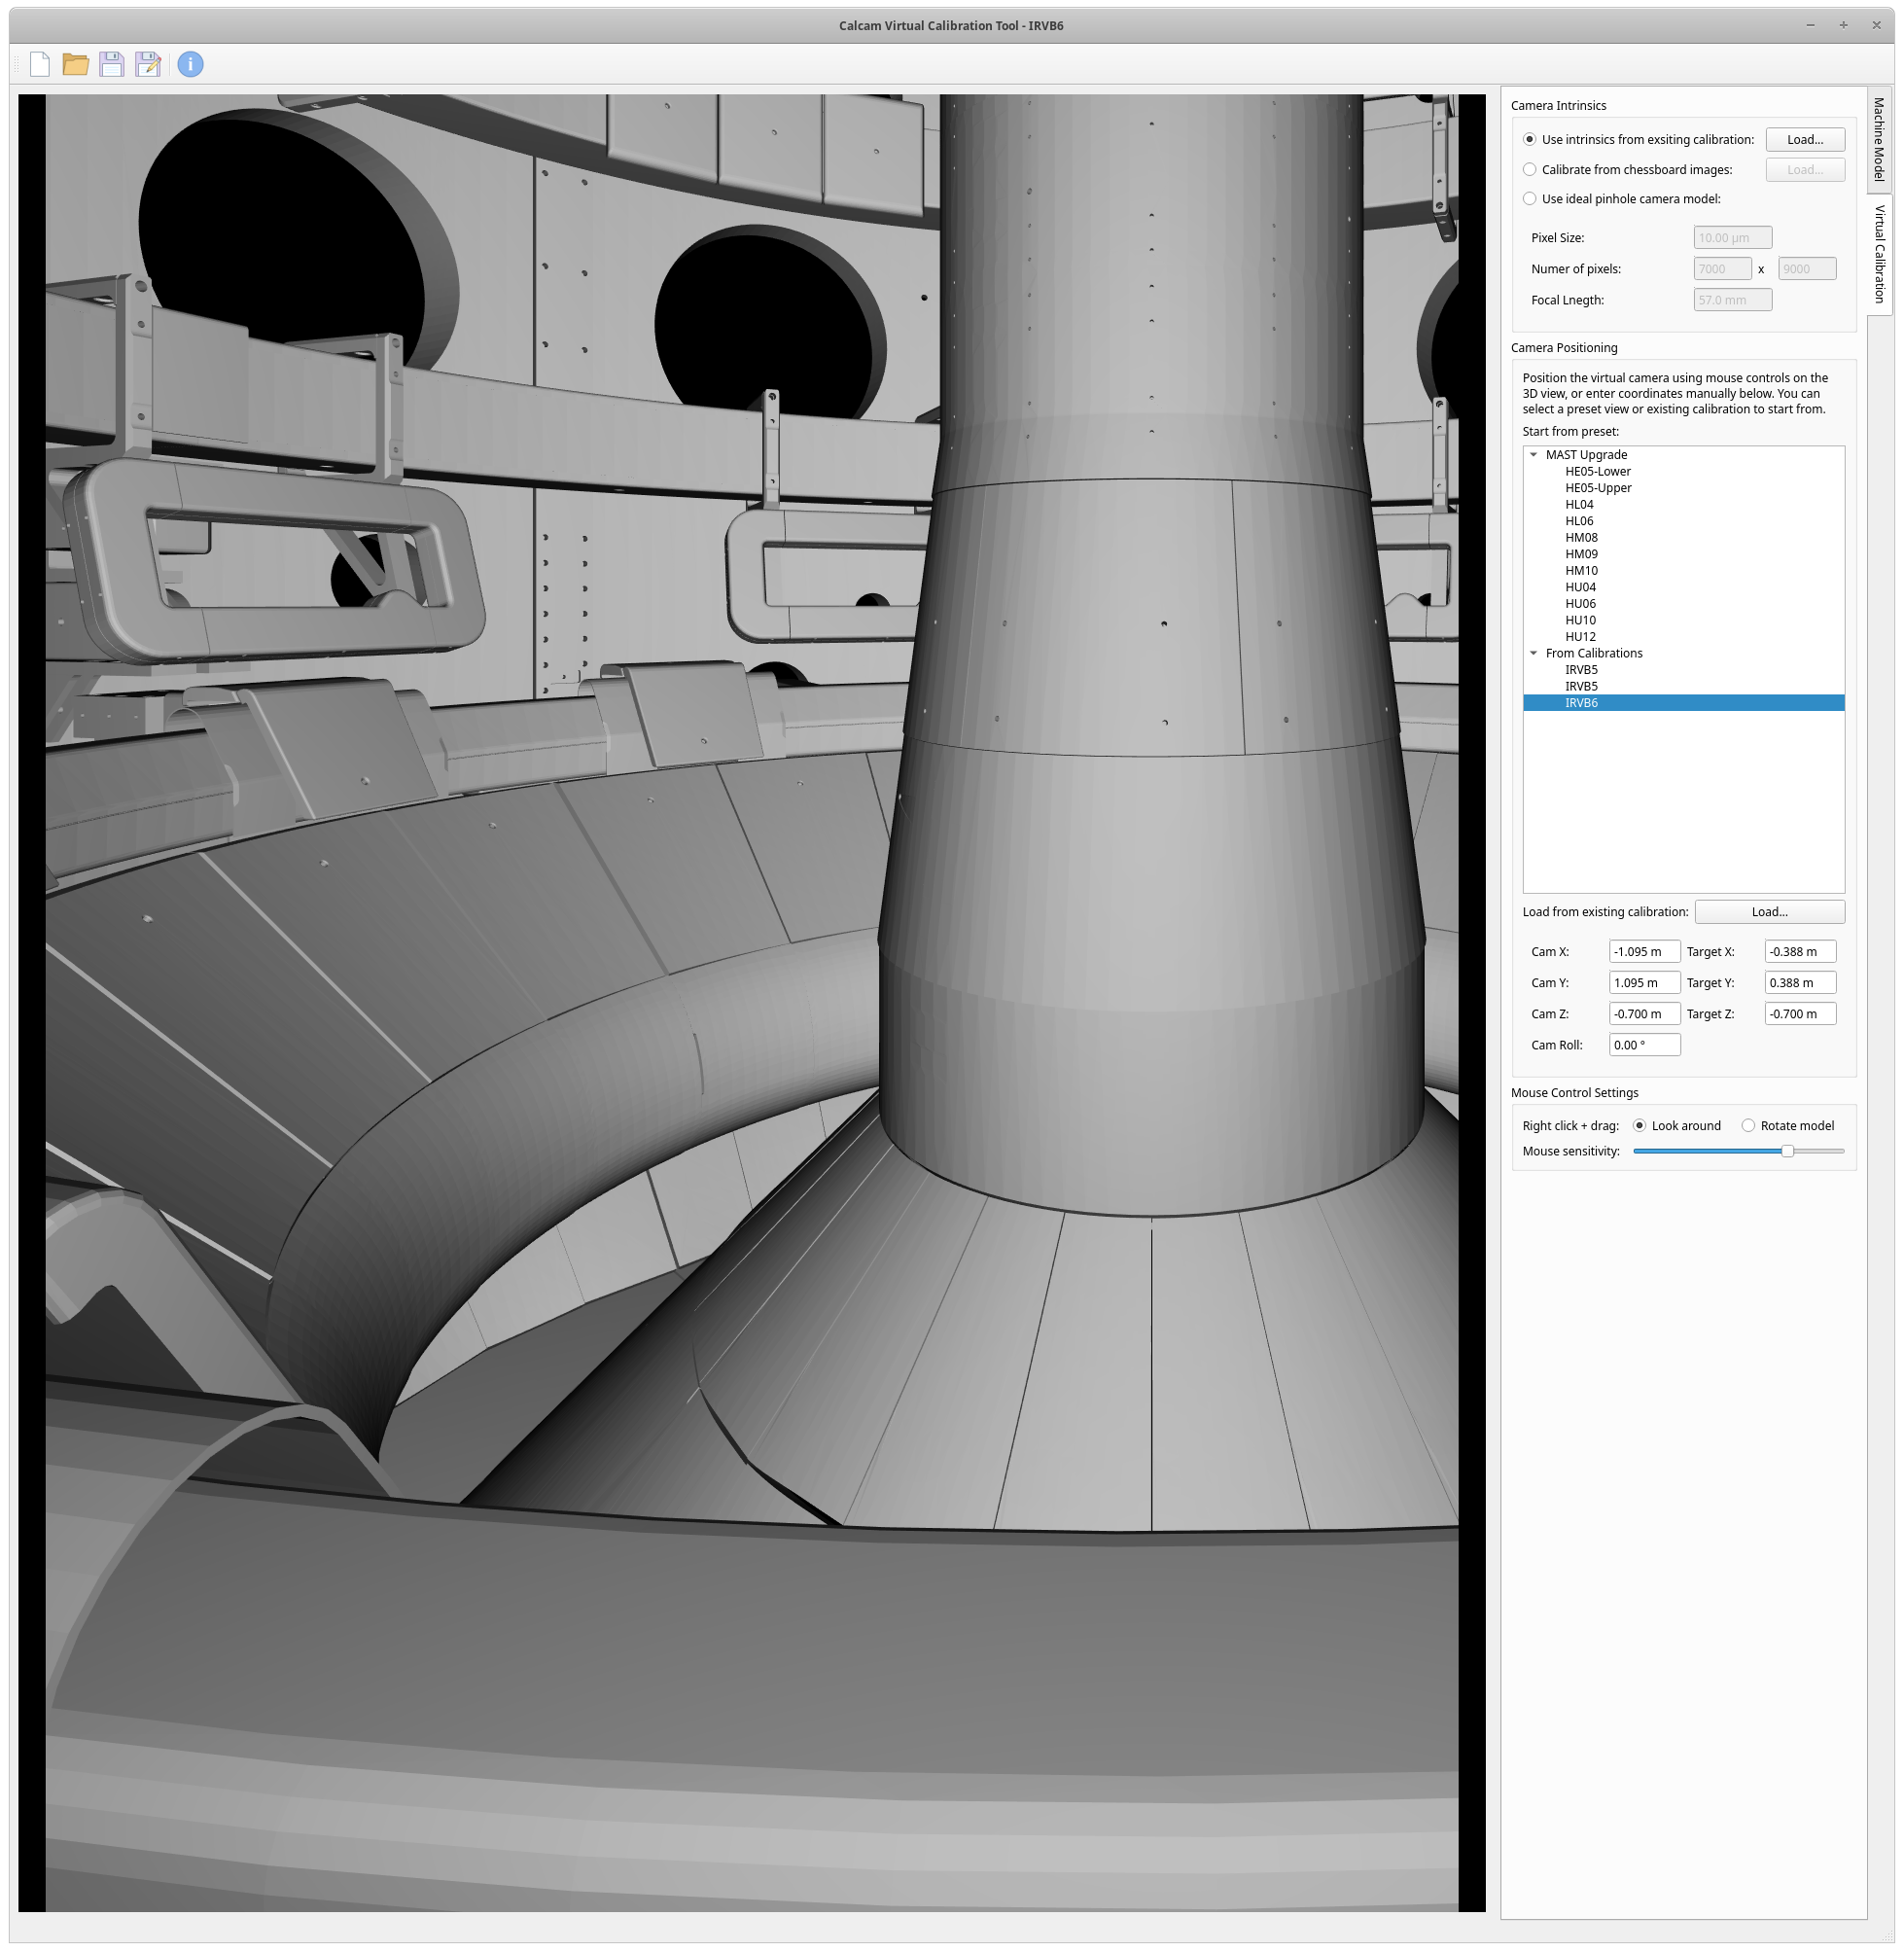
\includegraphics[trim={30 10 450 85},clip,width=0.6\linewidth]{Chapters/chapter2/figs/calcam.png}
	\caption{Approximate view inside MASTU as if the IRVB operates as a camera.}
	\label{fig:calcam}
\end{figure}

The foil is a 2.5$\mu$m thick platinum foil. The thickness is optimised to stop photons with energies up to 8.2keV. \cite{PETERSON2010} The foil and its support frame have been spray blackened on both sides with Aerodag® G Graphite Aerosol and calibrated with a procedure analogous to the one exposed in \cite{Itomi2014}. The layer of graphite helps to absorb radiation in the visible range avoiding reflection and even if thicker that the platinum layer it is thermally less relevant. \cite{VanEden2018} The tube where the foil is installed is slightly larger than the frame and extends from the the vacuum chamber wall to a position close to the plasma, but still safely outside the SOL. The camera, a FLIR SC7500, images the foil through a ZnS view port with anti reflection coating and is bolted to the tube. The camera is equipped with a 2.5-5$\mu$m filter and was selected among others as the same model was adopted for other diagnostics in MASTU and the same acquisition software could potentially be developed.
The pinhole and stand off definition was made based on the expected radiated power from the plasma estimated with CHERAB \cite{C.GiroudA.MeakinsM.CarrA.Baciero2018}\cite{Carr2017}\cite{A.MeakinsCarrM.2017}, a code that can perform ray tracing with the full geometry of MAST-U.  Based on the aforementioned design for NSTX-U it was expected a good Signal to Noise Ratio (SNR) for a power density on the foil above $100W/m^2$ and a noise floor of about $5W/m^2$. \cite{Reinke2018} 

The tube was installed on MAST-U in November 2018 while all parts outside the vacuum vessel by early 2021. The calibration of the system was performed part in 2018 and part after the end of the first experimental campaign in late 2021. More detail on design considerations in \autoref{MASTUdesign}.


\section{Numerical technique}
To obtain the total radiated power profile a number of steps must be followed. \autoref{fig:numerical_path} shows in the bottom section the necessary steps.

\begin{figure}
	\centering
	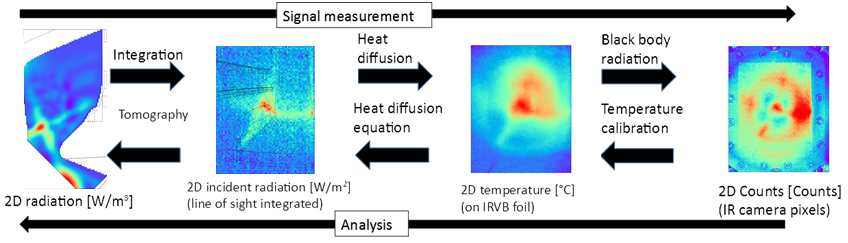
\includegraphics[width=\linewidth]{Chapters/chapter2/figs/numerical_path.png}
	\caption{Path for forward modeling, left to right, and for experimental data analysis, right to left.}
	\label{fig:numerical_path}
\end{figure}
I will now illustrate each step. More detail on the calibration procedure to obtain the necessary coefficients is provided in \autoref{IRVBcalibration}.

\subsection{Temperature calibration}
The temperature calibration is the procedure used to convert the camera row data from counts to temperature. It involves defining the mathematical model for the conversion and finding the coefficients required. Once defined it can be applied to MASTU data to obtain the IRVB foil temperature.
The surface of the foil is approximated as a black body emitter. The photons emitted by a BB source within the camera integration time can be modelled as \autoref{eq:BBphotons1}


\begin{equation}
{\Phi}_p (T) = \epsilon i \int_{ {\lambda}_1 }^{ {\lambda}_2 } {\frac{2 \pi c } { {\lambda}^4 } \frac {1} { e^{\frac {hc} {\lambda k T}} -1} {d \lambda} }
\label{eq:BBphotons1}
\end{equation}

with $\epsilon$ emissivity, $i$ integration time, $\lambda$ wavelength and $\lambda_1-\lambda_2$ the range allowed by the camera filter and $T$ the surface temperature.
To simplify the calculations an interpolator is built such that

\begin{equation}
\frac {{\Phi}_p (T)} {T} = \alpha (T) , T = {\alpha}_r ({\Phi}_p)
\label{eq:BBphotons2}
\end{equation}

The number of photons reaching the camera are going to be proportional to the number of emitted photon, with an additional offset due to thermal photons originated from other solid surfaces and the air. This offset will be approximately constant because it will not depend on the surface temperature observed by the camera.
The presence of the view port between camera and the source of BB radiation will decrease the number of thermal photons reaching the camera and potentially modifies the constant offset.
Assuming that the number of counts is proportional to the number of photons, and that this does not depends on the photon wavelength, the number of camera counts can be expressed as:

\begin{equation}
C = a_1 \cdot a_3 \cdot {\Phi}_p (T) + a_2 + a_4
\label{eq:BBphotons3}
\end{equation}

with $a_1\in[0,\infty]$ and $a_2\in[-\infty,\infty]$ the proportional and constant component for the counts without the window and $a_3\in[0,1]$ and $a_4\in[-\infty,\infty]$ the modifiers for the window case. $T_0$ and $C_0$ are the temperature and counts relative to the initial conditions at the beginning of the shot (room temperature).
In order to calculate all 4 coefficients 2 temperature ramps are required, one with and one without window. When changing the temperature of the BB source the camera counts have to be monitored to make sure to collect the data only after they have stabilised.
The counts/temperature curves obtained are then fit to return the coefficients. The power absorbed by the IRVB foil is obtained using the temperature increase over the profile before the pulse ($T_0$ and $C_0$), so the constant offset from the calibration will not impact the results while it does for the uncertainty, even if usually negligibly.
Once $a_1 \cdot a_3$ is determined the temperature is calculated as:

\begin{equation}
T = {\alpha}_r ( {\Phi}_p(T)) = {\alpha}_r \left (\frac {C - a_2 - a_4} {a_1 \cdot a_3} \right ) = {\alpha}_r \left (\frac {C - C_0} {a_1 \cdot a_3} + {\Phi}_p (T_0) \right )
\label{eq:BBphotons4}
\end{equation}

At this stage the temperature is binned appropriately to increase signal to noise. In most circumstances it was adopted a binning of 12-14 temporal steps and 3x3 pixels.

\subsection{Foil calibration}
The foil thermal response is dictated by heat transport having as source the radiated power from the plasma and as sinks its black body radiation and conduction to the frame. The foil is very thin and therefore 2D heat transport can safely be considered instead of 3D. \autoref{eq:heat2d} shows how to calculate the power absorbed by the foil based on its temperature.

\begin{equation}
\begin{split}
P_{foil}= P_{\frac {\partial T} {\partial t}}+P_{\Delta T}+P_{BB}\\
P_{\frac {\partial T} {\partial t}}=k \: t_f \: \dfrac{1}{\kappa} \dfrac{dT}{dt} \\
 P_{\Delta T} = -k \: t_f \:  \left( \dfrac{\partial^2 T}{\partial x^2} + \dfrac{\partial^2 T}{\partial y^2} \right) \approx -k \: t_f \: L \cdot T \\ P_{BB} = 2 \: \varepsilon \: \sigma_{SB} \: (T^4 - T_0^4)
\label{eq:heat2d}
\end{split}
\end{equation}

with $k$ thermal conductivity, $t_f$  thickness, $\kappa$ thermal diffusivity, $\varepsilon$ black body emissivity and $\sigma_{SB}$ the Stefan-Boltzmann constant. $L$ is the matrix containing the coefficients to build the temperature Laplacian via the dot product. It is built such that by dot product with the temperature it returns the sum of the second order central finite difference in all directions.

The uncertainty on the temporal variation, diffusion and radiation terms of the heat equation can be calculated with \autoref{eq:uncert1}, \ref{eq:uncert2} and \ref{eq:uncert3} respectively
\begin{equation}
{\sigma }_{ \frac {\partial T} {\partial t}} = \frac 1 {dt}  \sqrt{ \left ( \frac {{\sigma }_{C_{i+1}}} { a_1 a_3 \alpha(T_{i+1}) } \right )^2 + \left ( \frac {{\sigma }_{C_{i-1}}} { a_1 a_3 \alpha(T_{i-1}) } \right )^2 + \left [ \left ( T_{i+1}-T_{i-1} \right ) \frac {{\sigma }_{a_1 a_3}} {a_1 a_3} \right ]^2 } 
\label{eq:uncert1}
\end{equation}
\begin{equation}
{\sigma }_{ \Delta T} = \frac {1} {dx^2} \sqrt{ L^2 \cdot \left[  \left(  \frac {{\sigma }_{C_i}} { a_1 a_3 \alpha(T_i) } \right)^2 + \left( \frac {{\sigma }_{C_0}} { a_1 a_3 \alpha(T_0) } \right)^2 + \left( ({T_i -T_0}) \frac {{\sigma }_{a_1 a_3}} {a_1 a_3} \right)^2 \right] } 
\label{eq:uncert2}
\end{equation}\begin{equation}
\begin{split}
{\sigma }_{T_i} = \frac 1 {\alpha(T_i)} \sqrt{ \frac {({\sigma }_{C_i}^2 + {\sigma }_{C_0}^2 )} { (a_1 a_3)^2 } + \left [ \left (\frac {C_i -C_0} {a_1 a_3} \right ) \frac {{\sigma }_{a_1 a_3}} {a_1 a_3} \right ]^2  + (\alpha(T_i) {\sigma }_{T_0})^2 } \\ {\sigma }_{ BB} = 4 \sqrt{ ({T_i}^3 {\sigma }_{T_i})^2 + ({T_0}^3 {\sigma }_{T_0})^2 }
\label{eq:uncert3}
\end{split}
\end{equation}


\subsection{Tomography}
Assuming the radiation from every voxel of the plasma is assumed to be emitted uniformly and the opacity of the plasma itself is neglected \hl{[reference]} the relation between emissivity map $m$ and power to every pixel of the foil $q$ is linear and can be summarised in the matrix product

\begin{equation}
Gm=q
\label{eq:gmq}
\end{equation}

Scanning the voxels with a known emitter it is possible to determine all the elements of the matrix $G$, the geometry matrix. For this work this was done with the Monte Carlo ray tracing code CHERAB. To obtain the emissivity map from the power on the foil the geometry matrix must be inverted, but this is an ill-posed problem. A problem is well posed if a solution exists, it is unique and it has small changes for small changes of the inputs. \cite{Hansen1998} In the case of tomographic inversions often the last condition fails. \cite{Hansen2010} This means additional information have to be added in order to find a solution. In the most famous case of tomographic inversion, MRI scans, the source and detector are moved around the volume of interest as to collect information from different angles. This decreases the under-determination of the problem and a solution can be found. In our case neither observer or observed can be moved so additional information are required for a stable solution.
\subsection{Literature}
\subsubsection{Truncated singular value decomposition}
The truncated singular value decomposition (SVD) method for tomographic inversion relies of the direct inversion of the geometry matrix. The inversion is performed by finding the eighenvalues and eighenvectors associated with the geometry matrix. The matrix inversion can often be numerically performed, but the smaller eighenvalues greatly enhance the effect of any noise in the measured data and even numerical rounding errors. This can be limited by neglecting the smaller eighenvalues (hence truncating) and to consider only the more significant ones.
\subsubsection{Tikhonov regularization}
With this method the synthetic image $Gm'$ is calculated and the norm of the residuals calculated. This can then be minimised to find the best precursor. Because this method is also effected by noise a penalty is added to limit its effect. There are various choices for what to limit exactly, but the most common is to limit a derivative of the solution from the zero-th order (limitation on large values) to second (limitation of the laplacian). In this work the laplacian penalty is considered. The derivative is multiplied by a regularisation coefficient in determining the penalty. The sum of the penalty and the residuals norm is then minimised. \cite{Schou2015} This method is simple but numerically demanding for large number of voxels. This can be alleviated by providing the Hessian matrix to the solver, but is still onerous as large matrices have to be handled.
\subsubsection{Simultaneous algebraic reconstruction technique}
Simultaneous algebraic reconstruction technique (SART) is an iterative method that aims at minimizing the difference between the measurement $q$ and the synthetic image $Gm'$, and the difference at each step informs how to correct the previous guess. Here too the noise requires a penalty with relative regularisation parameter to be applied, but it is in general less computationally demanding than the previous method. SART can also be modified to avoid negative emissivity. Because of it's relative low computational cost this is often the method of choice when inverting imaging data from plasmas.

\subsection{Regularisation optimisation}
The regularisation method depends on the inversion method chosen. The goal is to find the best compromise between a smooth solution with a realistic profile and one that fits best the measured data.
\subsubsection{Eigenvalues truncation}
It is often observed that the eigenvalues associated with the geometry matrix, sorted by amplitude, behave as shown in \autoref{fig:eigenvalues}.

\begin{figure}
	\centering
	\includegraphics[trim={0 20 0 40},clip,width=\linewidth]{Chapters/chapter2/figs/eigenvalues_for_alpha_1e-30_2.eps}
	\caption{Typical amplitude of the eigenvalues in an undetermined inversion problem.}
	\label{fig:eigenvalues}
\end{figure}

In the process of inverting the geometry matrix the the reciprocal of the eigenvalues is used. This means that the smaller of them, that have the lesser influence on the measured data, have a disproportionate effect on the solution. To limit this the smaller eigenvalues can be neglected. How to find the threshold is not simple and it also depends on the noise level in the input data. In general truncated SVD returns more detailed inversions, but it is more effected by noise than other methods. More detail can be found in \cite{Schou2015} and \cite{Widman2002}.

\subsubsection{L-curve}
For the Tikinov and SART algorithms one has to establish the magnitude of the regularisation coefficient. A commonly used method is the L-curve. With this approach the emissivity solution is calculated for a range of regularisation parameters. The residuals norm and the norm of the penalty are plotted in a log-log plot to create the L-curve. A typical L-curve is shown in \autoref{fig:l-curve}.

\begin{figure}
	\centering
	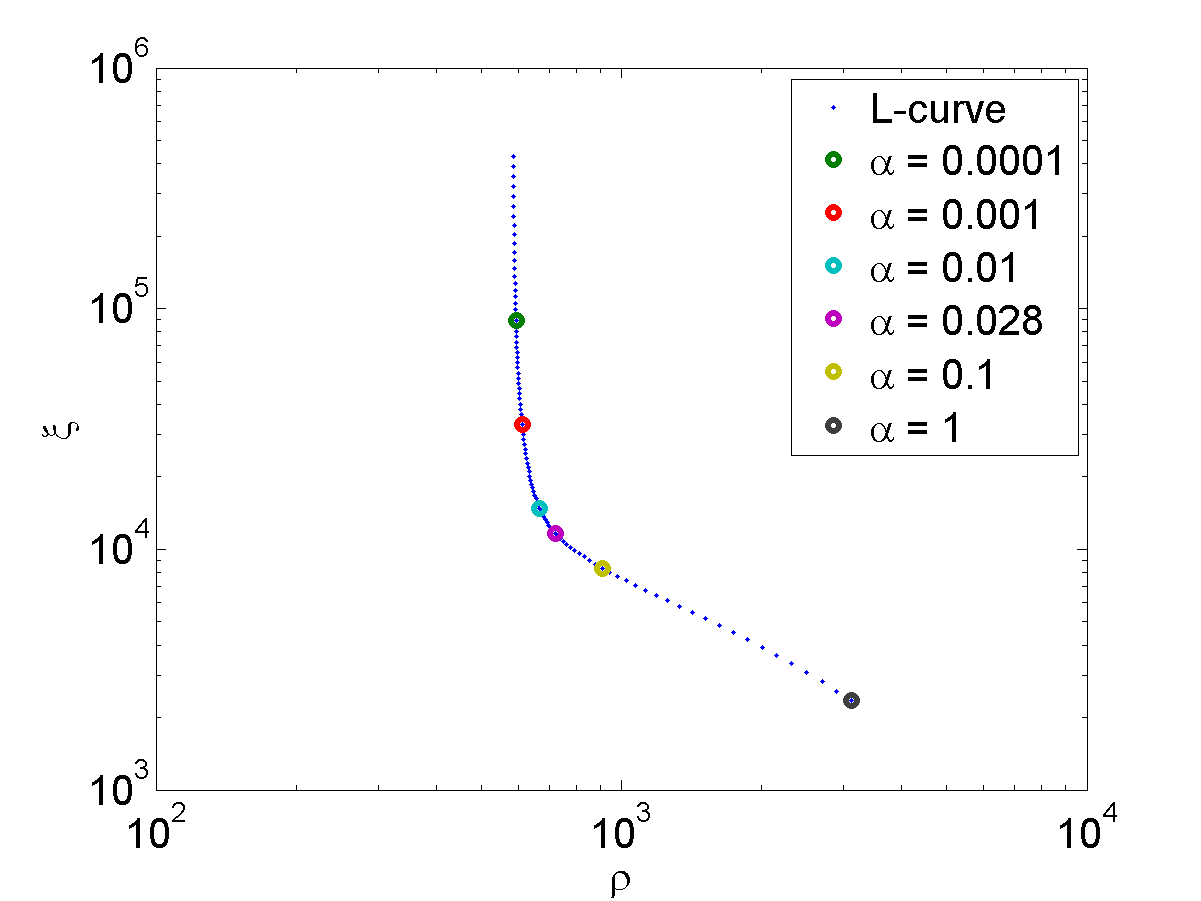
\includegraphics[width=\linewidth]{Chapters/chapter2/figs/l-curve.png}
	\caption{Typical L-curve shape. On the horizontal axis the residual norm, on the vertical the penalty norm. \hl{I will create my own plot}}
	\label{fig:l-curve}
\end{figure}

The optimal solution is one that fits well the measured data but is not dominated by noise. A good compromise corresponds to the lower left corner of the curve, the region of highest curvature. This procedure requires a multitude of solution to be found for each inversion, but guarantees that the regulatisation is always adequate to the signal strength.
\subsection{Novelty (is it?): Bayesian approach with regularization}
This approach was developed specifically for the IRVB in MASTU and it is similar to Tikhonov regularisation. The residual norm is calculated this time including the uncertainty of the measurement in each pixel. Penalties can be simply included by adding them to the residuals norm. The following are included:
\begin{itemize}
\item laplacian of the emissivity
\item negative emissivity values
\item emissivity close to the pinhole
\end{itemize}
Additionally two variables are included: a uniform power density value over the whole foil and one only over the region of the foil actually effected by the plasma (see \autoref{fig:cherab2}). This is done to allow for uniform signal arising from a change of the IR camera temperature or sensitivity or sources of radiation close to the pinhole to be accounted for and not effect the emissivity distribution.
To alleviate the computational cost of the method the derivative of the quantity to minimise respect to all variables (emissivity in every pixel and offsets) is generated. The minimisation was operated with the L-BFGS-B algorithm, specifically the Python scipy.optimize.fmin\_l\_bfgs\_b package. \cite{Morales2011}
By varying the regularisation coefficient an L-curve is built and the point of maximum curvature found.
Every penalty should be provided of an individual coefficient and an L-curve built to find its optimal value, but because it would be computationally prohibitively onerous a coefficient that returns the desired result is determined a priory.\\
\hl{add all the math}
\subsection{Comparison with other methods}
The most commonly used inversion algorithms are Tikonov regularisation and SART. The optimisation of the regularisation coefficient is sometimes neglected, but for a fair comparison I will use the L-curve method.\\
\hl{to be done}

\section{first MASTU experimental campaign results}
\subsection{Movement of peak radiation with detachment}
\hl{ACTUAL OBSERVATION}\\
In discharges in which the core density was progressively increased, both via fuelling from the midplane or the divertor, the emissivity peak moves first from the inner target, then from the outer one, to the x-point. Increasing the density further the radiation moves upstream on the inner separatrix.
In lower power discharges the inner target has a comparatively much lower emissivity than the outer target, even if the sequence of events remains the same, and the transition on the inner leg seems significantly faster.
See \autoref{fig:44892} and \autoref{fig:45401}.

\begin{figure}
     \centering
     \begin{subfigure}{0.21\textwidth}
         \centering
         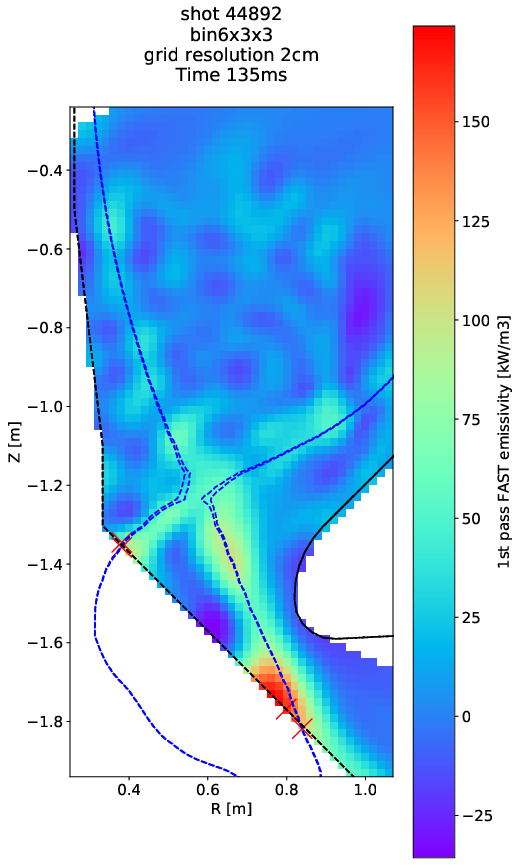
\includegraphics[trim={0 0 25 0},clip,width=\textwidth]{Chapters/chapter2/figs/44892_1.png}
         %\caption{pinhole 4mm/stand-off 45mm}
         \label{fig:44892_1}
     \end{subfigure}
     \hfill
     \begin{subfigure}{0.2\textwidth}
         \centering
         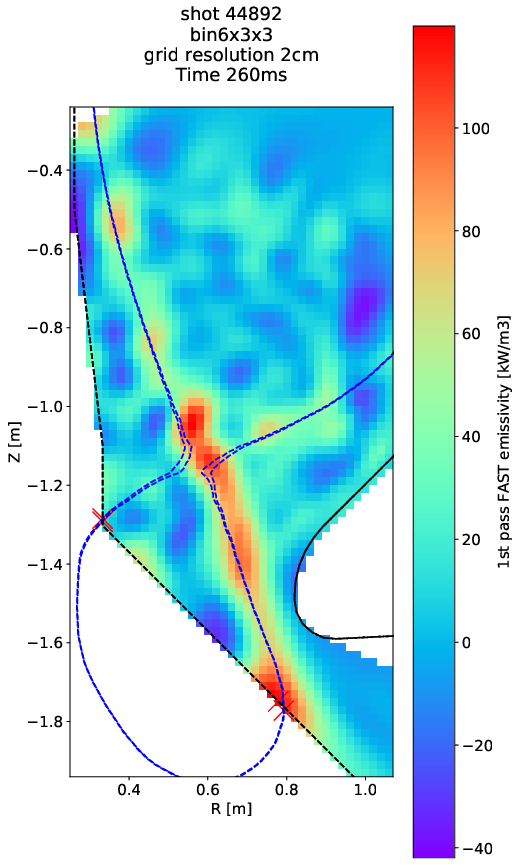
\includegraphics[trim={70 0 25 0},clip,width=\textwidth]{Chapters/chapter2/figs/44892_2.png}
         %\caption{$4/60$}
         \label{fig:44892_2}
     \end{subfigure}
     \hfill
     \begin{subfigure}{0.2\textwidth}
         \centering
         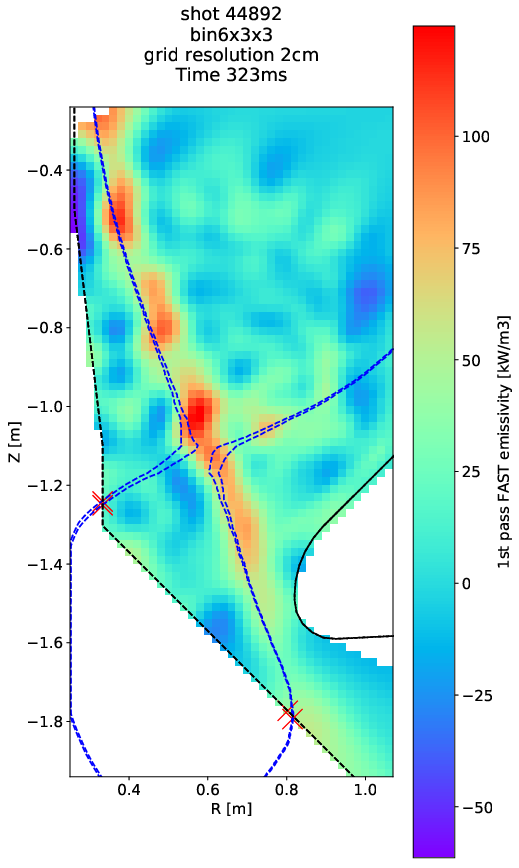
\includegraphics[trim={70 0 25 0},clip,width=\textwidth]{Chapters/chapter2/figs/44892_3.png}
         %\caption{$4/60$}
         \label{fig:44892_3}
     \end{subfigure}
     \hfill
     \begin{subfigure}{0.21\textwidth}
         \centering
         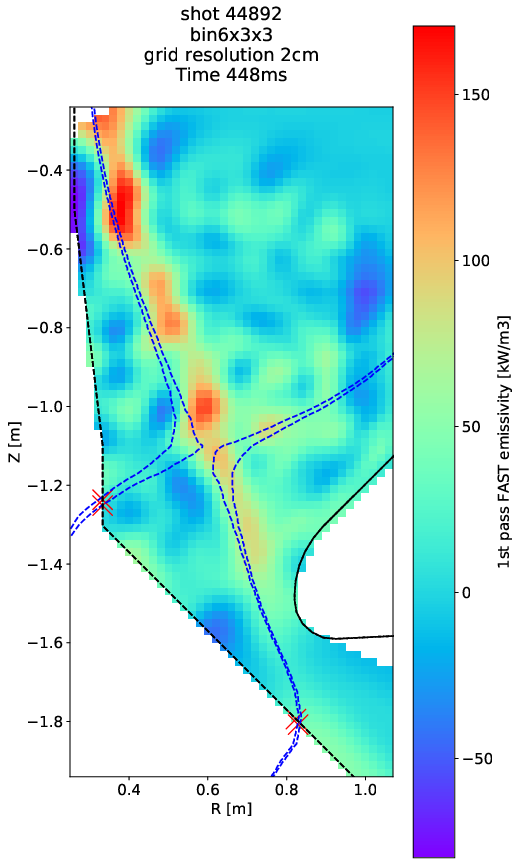
\includegraphics[trim={70 0 0 0},clip,width=\textwidth]{Chapters/chapter2/figs/44892_4.png}
         %\caption{$4/60$}
         \label{fig:44892_4}
     \end{subfigure}
    \caption{Changes in emissivity pattern from a attached plasma (left) to a detached one (right) in a low power discharge (shot 44892, DN-600-CD-OH, L-mode)}
    \label{fig:44892}
\end{figure}

\begin{figure}
     \centering
     \begin{subfigure}{0.21\textwidth}
         \centering
         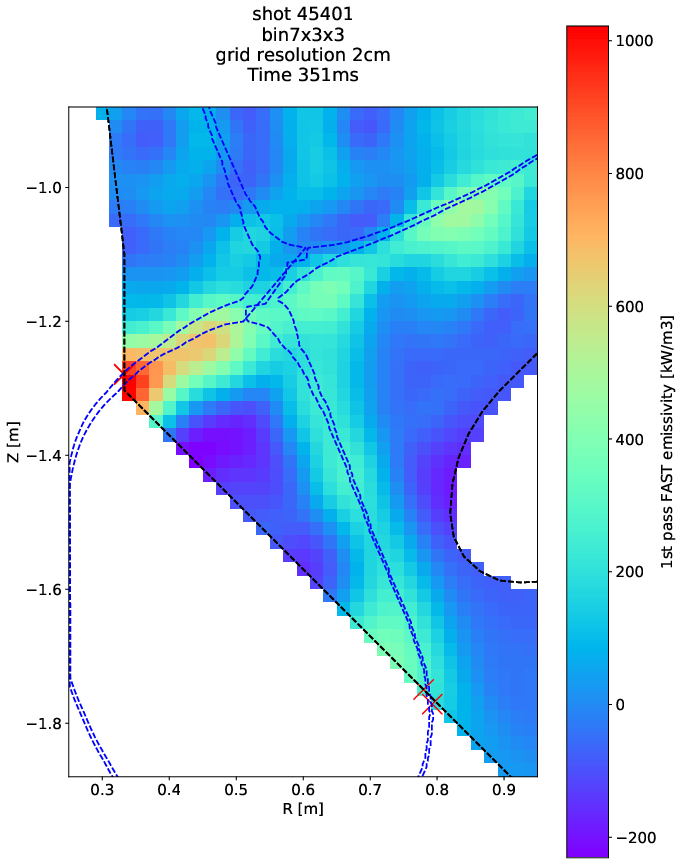
\includegraphics[trim={0 0 25 0},clip,width=\textwidth]{Chapters/chapter2/figs/45401_1.png}
         %\caption{pinhole 4mm/stand-off 45mm}
         \label{fig:45401_1}
     \end{subfigure}
     \hfill
     \begin{subfigure}{0.2\textwidth}
         \centering
         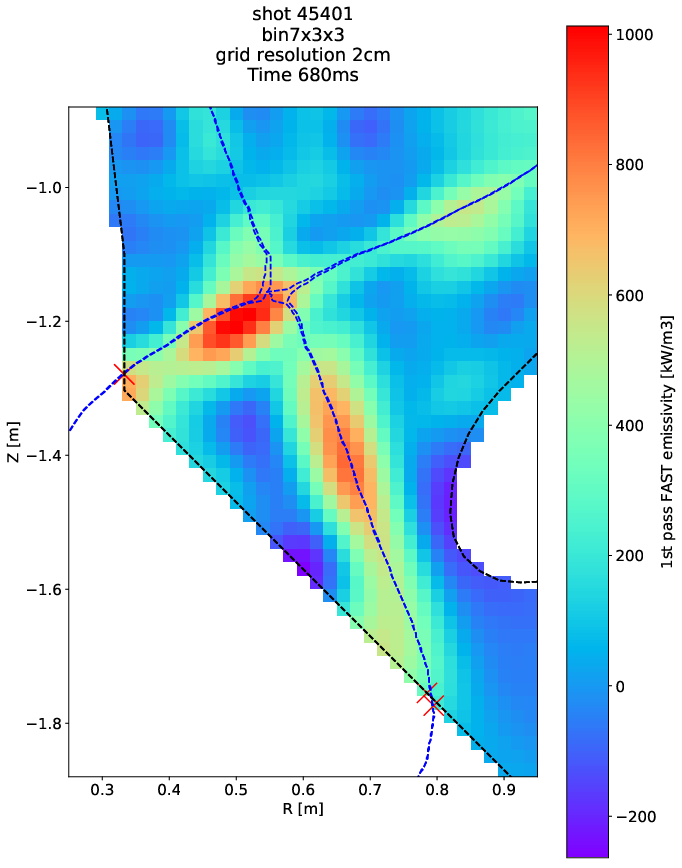
\includegraphics[trim={70 0 25 0},clip,width=\textwidth]{Chapters/chapter2/figs/45401_22.png}
         %\caption{$4/60$}
         \label{fig:45401_22}
     \end{subfigure}
     \hfill
     \begin{subfigure}{0.21\textwidth}
         \centering
         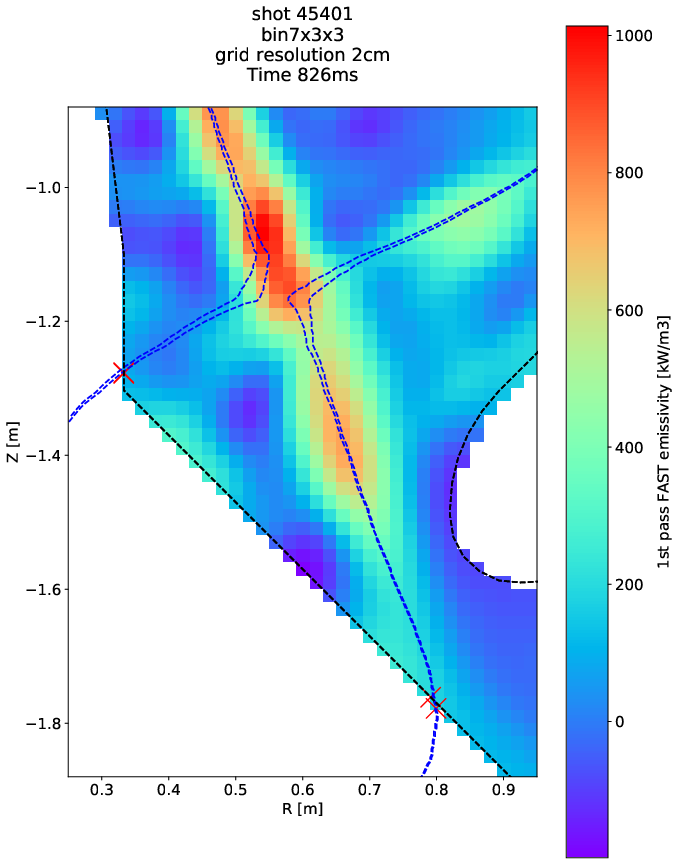
\includegraphics[trim={70 0 0 0},clip,width=\textwidth]{Chapters/chapter2/figs/45401_3.png}
         %\caption{$4/60$}
         \label{fig:45401_3}
     \end{subfigure}
    \caption{Changes in emissivity pattern from a attached plasma (left) to a detached one (right) in a high power discharge (shot 45401, DN-750-CD-2B, H-mode).}
    \label{fig:45401}
\end{figure}

\subsection{Detachment of SXD plasmas}
\hl{ACTUAL OBSERVATION}\\
As mentioned before the LOS entering the SXD chamber are too close to actually determine the emissivity distribution inside of it, but it is still possible to determine changes in the total radiated power. In \autoref{fig:45371} it is shown the change in total radiated power for a SXD discharge that experiences radiative detachment of the outer leg. Initially the total power radiated from the outer leg (simply defined as the region with $r>r_{X-point}, z<z_{X-point}$) and the SXD chamber grow together, with the part inside the chamber being the main contributor. Then after 0.4s the total in the whole leg remains stationary while it decreases in the chamber. This means that the radiation shifts in time upstream towards the x-point for increasing density.

\begin{figure}
     \centering
     \begin{subfigure}{0.21\textwidth}
         \centering
         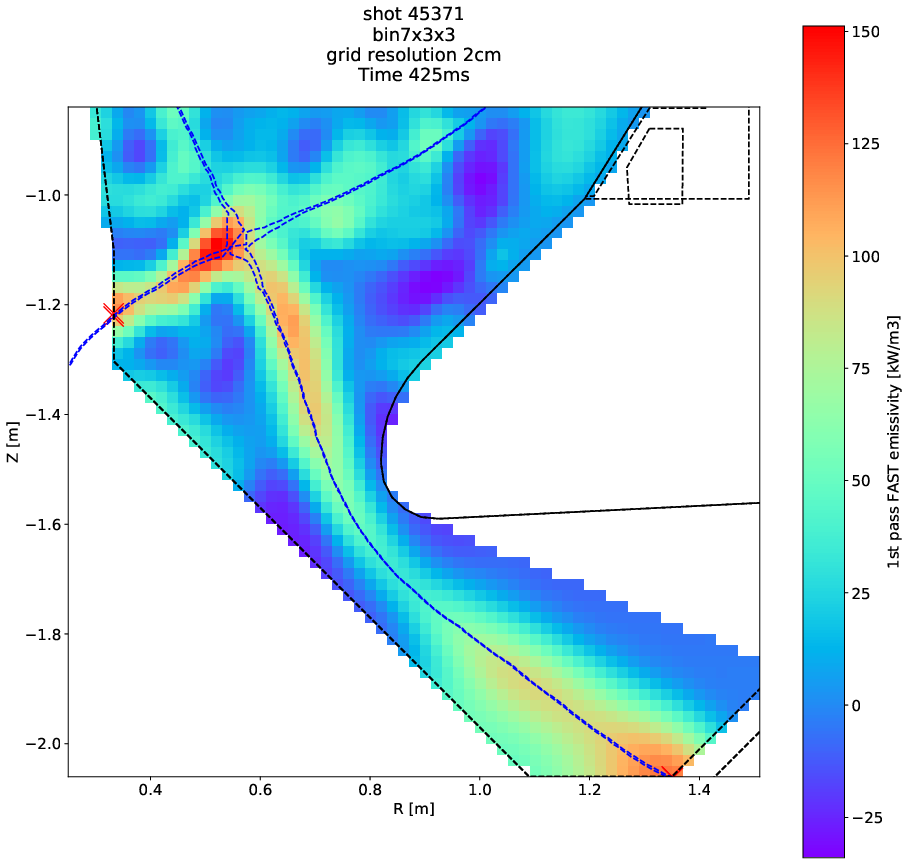
\includegraphics[trim={0 0 25 0},clip,width=\textwidth]{Chapters/chapter2/figs/45371_1.png}
         \caption{target attached\\(425ms)}
         \label{fig:45371_1}
     \end{subfigure}
     \hfill
     \begin{subfigure}{0.21\textwidth}
         \centering
         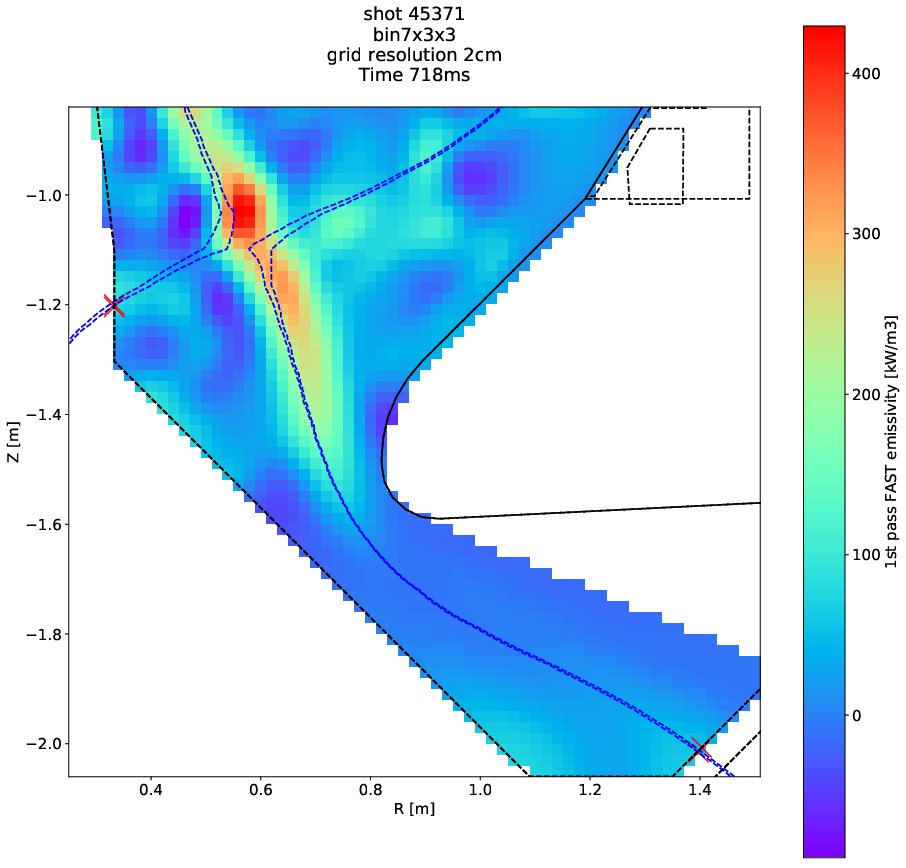
\includegraphics[trim={70 0 0 0},clip,width=\textwidth]{Chapters/chapter2/figs/45371_2.png}
         \caption{target detached\\(718ms)}
         \label{fig:45371_2}
     \end{subfigure}
     \hfill
     \begin{subfigure}{0.5\textwidth}
         \centering
         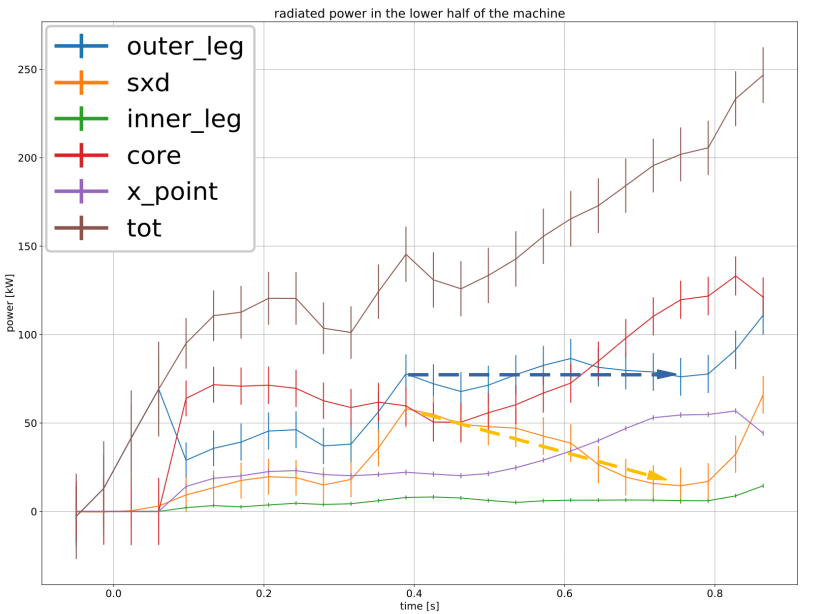
\includegraphics[trim={0 0 0 0},clip,width=\textwidth]{Chapters/chapter2/figs/45371_3.png}
         %\caption{$4/60$}
         \label{fig:45371_3}
     \end{subfigure}
    \caption{Changes in emissivity pattern for a SXD discharge where the detachment of the outer leg can be inferred from the change in total radiated power in the outer leg and SXD chamber (shot 45371, DN-600-SXD-OH, L-mode).}
    \label{fig:45371}
\end{figure}

\subsection{XPR/radiation location and confinement}
\subsection{XPR/detachment and power balance}
\subsection{radiation front location and analytic models}
\subsection{detachment and configuration (CD/SXD)}
CD more easily attached, need to compare 2 similar cases and radiation
different inner/outer detachment?
\subsection{radiation location and other metric of detachment}
radiation exits the divertor together with ionisation (from spectroscopy) $->$ hydrogen radiation dominant
with HFS fuelling tot rad peaks in inner separatrix?
compare resistive bolometer at x-point and IRVB: the resistive bolometer is not blackened to there could be a difference in sensitivity depending on the source of radiation.
\subsection{XPR and ELMs}
already found shots that start attached with ELMs and they stop with detachment, need to compare with radiation
